\thispagestyle{cackithitoannone}
\pagestyle{cackithitoan}
\everymath{\color{cackithi}}
\graphicspath{{../cackithi/pic/}}
\blfootnote{\color{cackithi}$^1$Khoa Toán Đại học Osnabrueck, CHLB Đức.}
\begingroup
\AddToShipoutPicture*{\put(0,616){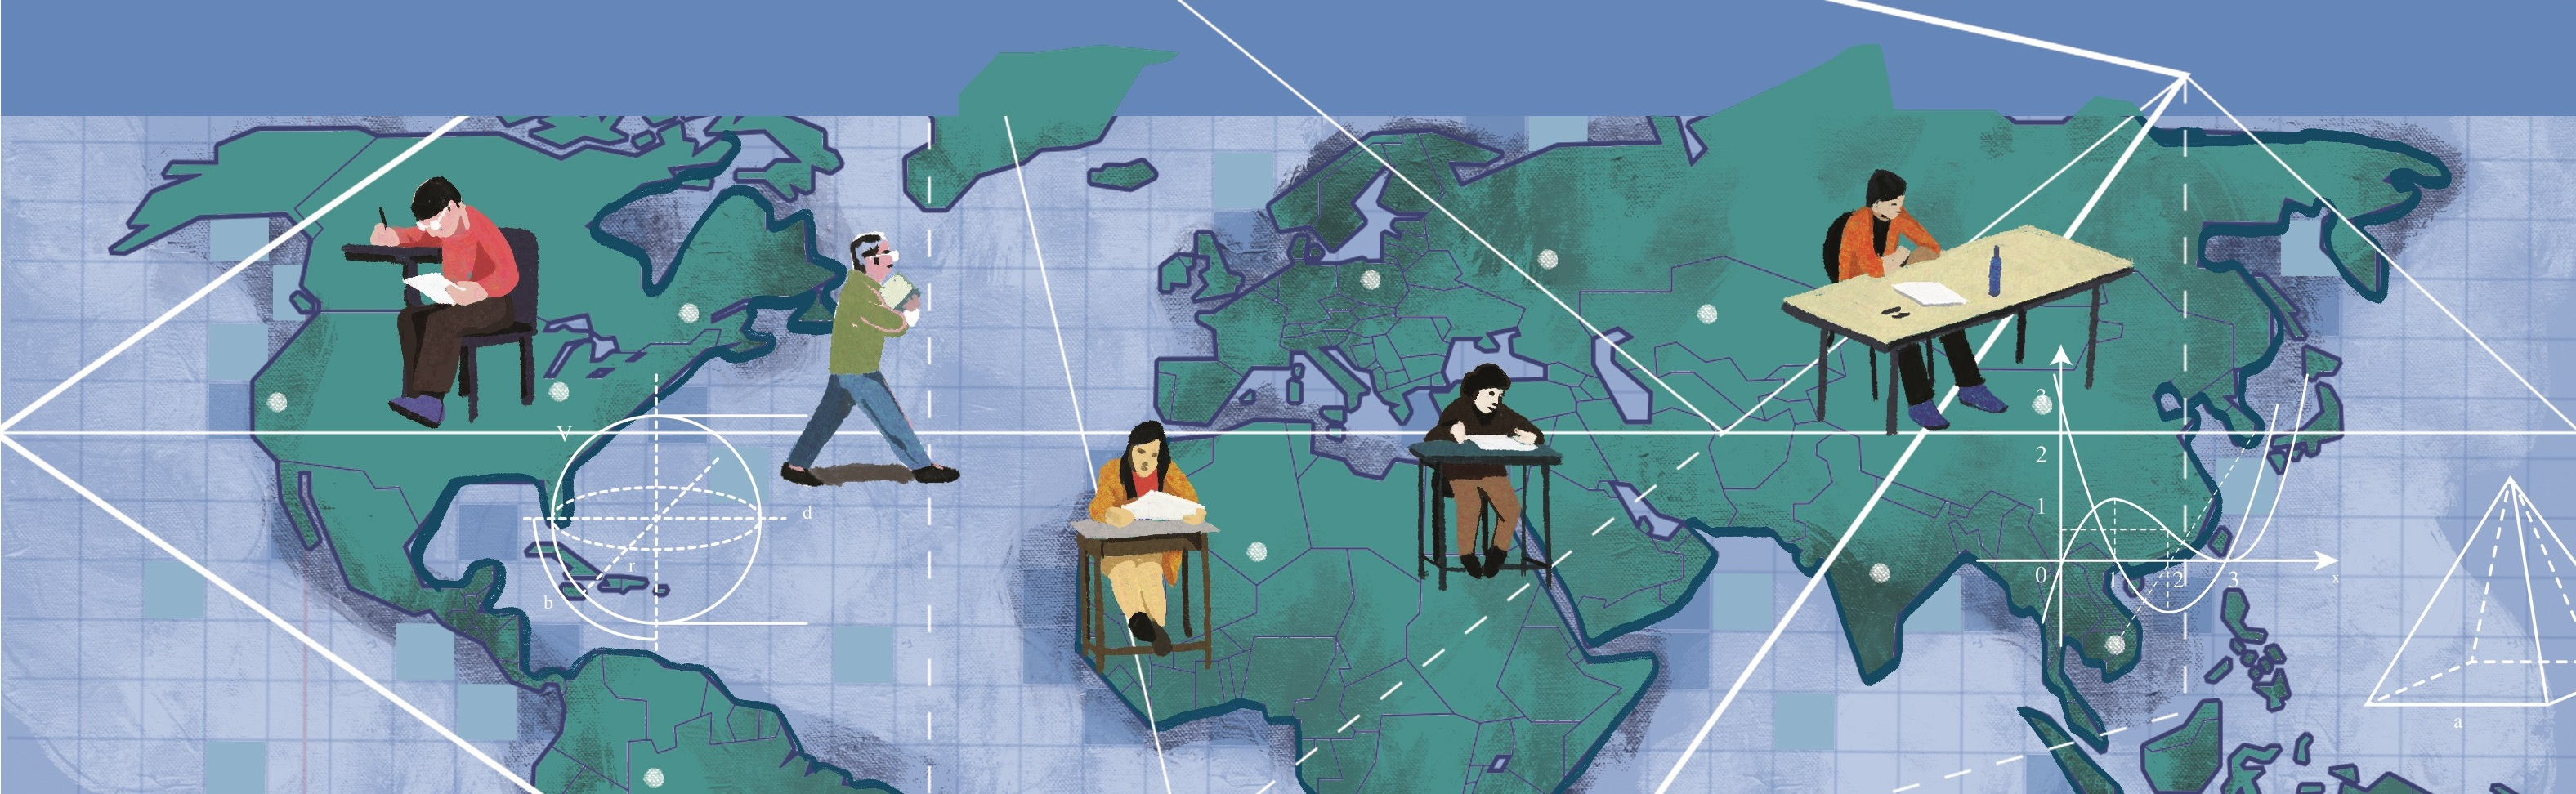
\includegraphics[width=19.3cm]{../bannercackithi}}}
\AddToShipoutPicture*{\put(82,527){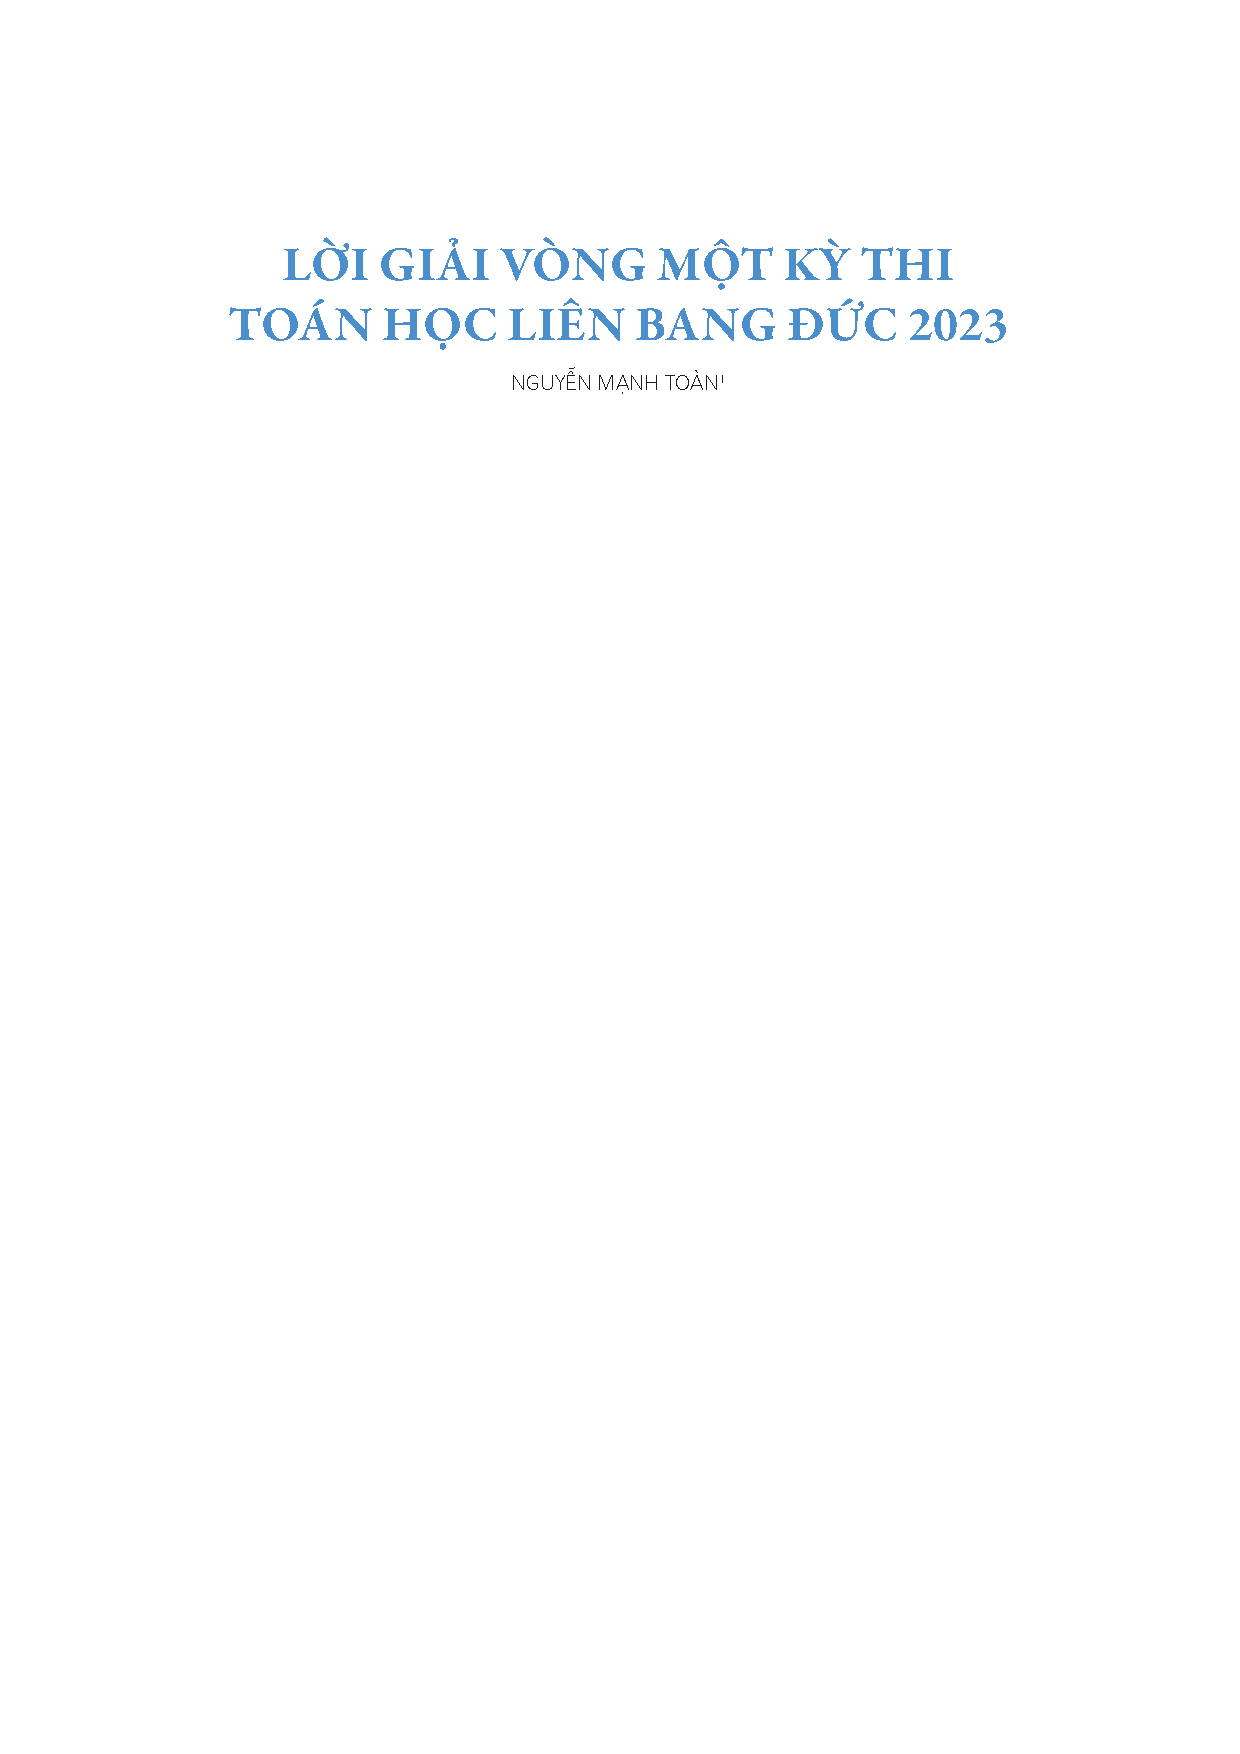
\includegraphics[scale=1]{../tieude2.pdf}}}
\centering
\endgroup
\vspace*{182pt}

\begin{multicols}{2}
	Trong chuyên mục này, chúng tôi sẽ trình bày Lời giải của các bài toán trong vòng một kỳ thi toán học liên bang Đức năm $2023$, đăng trong số báo $9/2023$. 
	\vskip 0.1cm
	\textbf{\color{cackithi}Câu $\pmb{1}$}: Ba bạn Tick, Trick và Track có $20$, $23$ và $25$ vé để đi vòng quay ngựa gỗ tại hội chợ hàng năm. Họ thống nhất rằng sẽ chỉ đi vòng quay nếu cả ba cùng đi và mỗi người nộp một vé của mình. Ngoài ra, trước mỗi lần đi, nếu muốn, họ có thể chia lại vé cho nhau bao nhiêu lần tùy thích theo quy tắc sau: Người nào có số vé chẵn thì có thể chia một nửa số vé của mình cho một trong hai người còn lại. Hỏi có thể xảy ra rằng sau một lần đi nào đó:
	\vskip 0.1cm
	$\bullet$ Đúng một người hết vé.
	\vskip 0.1cm
	$\bullet$ Đúng hai người hết vé.
	\vskip 0.1cm
	$\bullet$ Cả ba cùng hết vé. 
	\vskip 0.1cm
	\textit{Lời giải.}
	Để đơn giản ta sẽ biểu diễn phân bố vé bằng bộ ba số nguyên không âm, chẳng hạn ban đầu Tick, Trick và Track có $(20,23,25)$ vé.
	\vskip 0.1cm	
	$a.$ Có thể xảy ra trường hợp đúng một người hết vé. Chẳng hạn, nếu không bạn nào đưa vé cho bạn khác thì sau $20$ lượt đi Tick hết vé, Trick còn $3$ vé và Track còn $5$ vé.
	\vskip 0.1cm
	$b.$ Có thể xảy ra trường hợp đúng hai bạn hết vé. Chẳng hạn, sau $17$ lần đi thì số vé còn lại sẽ là $(3,6,8)$. Khi đó, Trick sẽ đưa một nửa số vé của mình, tức $3$ vé, cho Track và phân bố vé trở thành $(3,3,11)$. Sau $3$ lần đi tiếp thì Tick và Trick cùng hết vé còn Track còn $8$ vé.
	\vskip 0.1cm	
	$c.$ Không thể xảy ra trường hợp cả ba bạn hết vé đồng thời. Sau khi chuyển vé cho nhau thì tổng số vé của Tick, Trick và Track vẫn không đổi; tổng này chỉ giảm nếu cả ba đi cùng nhau và giảm đúng $3$ vé. Do vậy, để ba bạn cùng hết vé thì tổng số vé ban đầu phải là bội số của $3$. Tuy nhiên $20+23+25 = 68$ không chia hết cho $3$.
	\vskip 0.1cm
	\textbf{\color{cackithi}Câu $\pmb{2}$}: Tìm tất cả các bộ ba số nguyên $(x,y,z)$ thỏa mãn phương trình 
	\begin{align*}
		x^2 + y^2 + z^2 -xy-yz-zx = 3. \tag{$1$}
	\end{align*}
	\textit{Lời giải.}
	Nếu $(x,y,z)$ thỏa mãn phương trình ($1$) thì mọi hoán vị của bộ ba này cũng vậy. Do đó ta chỉ cần xét trường hợp $x \ge y \ge z$. Ta có
		\begin{align*} 
			&x^2 + y^2 + z^2 -xy-yz-zx  = 3 \\ 
			\Leftrightarrow	\,&2x^2 + 2y^2 + 2z^2 -2xy-2yz-2zx  = 6 \\
			\Leftrightarrow	\,&(x-y)^2 + (y-z)^2 + (x-z)^2  = 6. \tag{$2$}
		\end{align*}
		Với ba số nguyên không âm $a\ge b \ge c \ge 0$, phương trình $a^2 + b^2 + c^2 = 6$ có nghiệm khi và chỉ khi $a = 2$, $b = c = 1$. Từ giả sử ban đầu rằng $x \ge y \ge z$ ta có
		\begin{align*} 
			\Leftrightarrow
			\begin{cases}
				x - y = 1 \\
				y - z = 1 \\
				x - z = 2
			\end{cases} \Leftrightarrow
			\begin{cases}
				y = z + 1 \\
				x = z + 2.
			\end{cases}
		\end{align*}
		Do vậy, các bộ ba số nguyên liền nhau $(x,y,z) = (k+2, k + 1, k)$ và các hoán vị của chúng, với $k \in \mathbb{Z}$, là tất cả nghiệm nguyên của phương trình ($1$).
	\vskip 0.1cm
	\textbf{\color{cackithi}Câu $\pmb{3}$}: Cho hai hình bình hành $ABCD$ và $AECF$ có chung đường chéo $AC$, trong đó $E$ và $F$ nằm bên trong $ABCD$. Chứng minh rằng đường tròn ngoại tiếp của các tam giác $AEB$, $BFC$, $CED$ và $DFA$ giao nhau tại một điểm. 
	\vskip 0.1cm
	\textit{Chứng minh.}
	Gọi đường tròn ngoại tiếp các tam giác $AEB$, $BFC$, $CED$ và $DFA$ lần lượt là $k_1$, $k_2$, $k_3$ và $k_4$. Hai đường tròn $k_1$ và $k_3$ giao nhau tại $E$. Gọi giao điểm còn lại là $G$. Ta sẽ chứng minh rằng $G \in k_2$ và $G \in k_4$.
	\vskip 0.1cm		
	Gọi $S$ là trung điểm của đường chéo chung $AC$. Vì các hình bình hành đối xứng qua trung điểm của các đường chéo, điều kiện của bài toán có thể được mô tả đầy đủ thông qua các điểm $A$, $B$, $E$ và $S$. 
	\vskip 0.1cm		
	Giả sử có một đỉnh nào đó của $ABCD$ thuộc ba trong bốn đường tròn đã cho, chẳng hạn $B$ thuộc $k_1$, $k_2$ và $k_3$. Khi đó $G = B$. Vì $B$ nằm trên đường tròn $CED$ nên từ tính đối xứng tâm qua $S$ thì $D$ thuộc đường tròn $AFB$. Nói cách khác, $B \in k_4$ và bốn đường tròn $k_1$, $k_2$, $k_3$, $k_4$ đều đi qua $B$. Bởi vậy trong phần chứng minh dưới đây ta có thể giả sử rằng $G$ không trùng với đỉnh nào của $ABCD$.
	\vskip 0.1cm	
	\textit{Trường hợp $1$}: $G$ nằm ở phần trong hình bình hành $ABCD$. Khi đó $G$ và $E$ nằm cùng một phía với đường thẳng $AB$ cũng như cùng một phía với đường thẳng $CD$. Đặt
	\begin{align*}
		&\alpha \colon = \angle AEB = \angle CFD,\\
		&\beta \colon = \angle BEC = \angle DFA,\\
		&\gamma \colon = \angle CED = \angle AFB,\\
		&\delta \colon =  \angle DEA = \angle BFC.
	\end{align*}
	Do $E$ và $F$ nằm trong $ABCD$ nên $\alpha + \beta + \gamma + \delta = 360^{\circ}$.
	\vskip 0.1cm	
	Từ định lý về góc nội tiếp cho đường tròn $k_1$ với cung $AB$ ta có $\angle AGB = \angle AEB = \alpha$. Tương tự với đường tròn $k_3$ và cung $CD$ ta có $\angle CGD = \angle CED = \gamma$. Ta sẽ chứng minh rằng $\angle BGC = \delta = \angle BFC$. Vì $\alpha+ \beta + \gamma + \delta = \angle AGB + \angle DGA + \angle CGD + \angle BGC = 360^{\circ}$ nên từ đó suy ra $\angle DGA = \beta = \angle DFA$. Từ định lý về góc nội tiếp đường tròn $k_2$ với cung $BC$ và $k_4$ với cung $DA$ ta thu được $G \in k_2$ và $G \in k_4$. 
	\vskip 0.1cm	
	Xét ba trường hợp con có thể xảy ra:
	\vskip 0.1cm	
	\textit{Trường hợp $1a$}: Các điểm $A, G, E, B$ khác nhau đôi một và nằm trên đường tròn $k_1$ theo thứ tự kể trên. Khi đó, các điểm $D,G,E,C$ cũng nằm trên đường tròn $k_3$ theo thứ tự này và đoạn thẳng $GE$ nằm trong góc $\angle DEA$. Do đó, $\angle GED + \angle GEA = \angle DEA = \delta$.
	\begin{figure}[H]
		\vspace*{-5pt}
		\centering
		\captionsetup{labelformat= empty, justification=centering}
		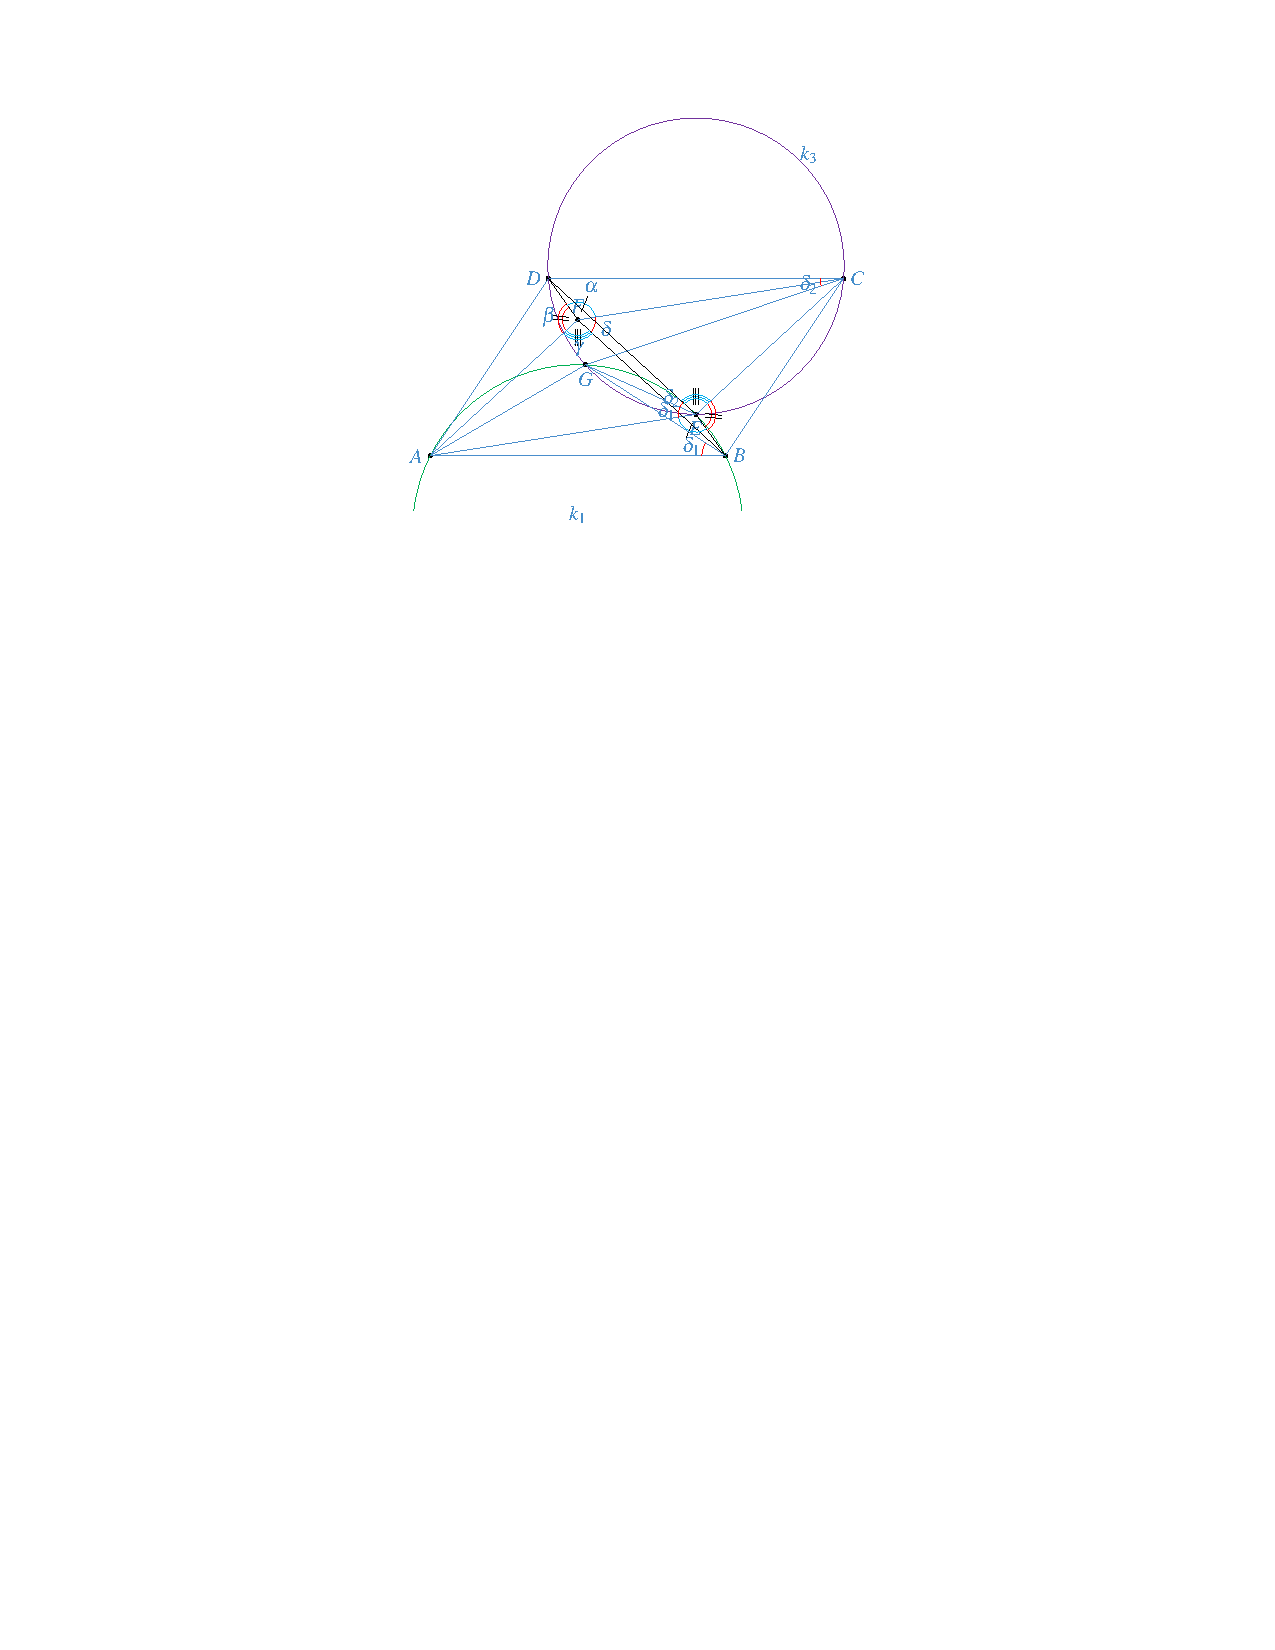
\includegraphics[width=1\linewidth]{h1}
		\caption{\small\textit{\color{cackithi}Hình $1$: Trường hợp $1a$.}}
		\vspace*{-10pt}
	\end{figure}	
	Từ định lý góc nội tiếp cho đường tròn $k_1$ với cung $AG$ và $k_3$ với cung $DG$ ta có $\angle GEA = \angle GBA$ và  $\angle GED = \angle GCD$. Do đó, $\angle GCD + \angle GBA = \delta.$
	\vskip 0.1cm	
	Vì $ABCD$ là hình bình hành nên
	$
	\angle GCB + \angle GCD + \angle GBA + \angle GBC
	= \angle DCB + \angle ABC
	= 180^{\circ}.
	$
	Do đó $\angle GCB + \angle GBC =  180^{\circ} - (\angle GCD + \angle GBA) = 180^{\circ} - \delta$.
	\vskip 0.1cm
	Mặt khác, vì $BGC$ là tam giác nên
	$
	\angle BGC + \angle GCB + \angle GBC = 180^{\circ}.
	$
	Do đó 
	$\angle BGC  = 180^{\circ} -(\angle GCB + \angle GBC)
	= 180^{\circ} - (180^{\circ} - \delta)  
	=  \delta
	$
	và ta có điều phải chứng minh.
	\vskip 0.1cm
	\textit{Trường hợp $1b$}: Các điểm $A, E, G, B$ khác nhau đôi một và nằm trên đường tròn $k_1$ theo đúng thứ tự kể trên. Khi đó lặp lại lý luận trong trường hợp 1a nhưng hoán đổi vị trí $A$ với $B$, $C$ với $D$ (do đó hoán đổi $\beta$ với $\delta$, $k_2$ với $k_4$, v.v...) ta thu được kết quả tương tự. 
	\begin{figure}[H]
		\vspace*{-5pt}
		\centering
		\captionsetup{labelformat= empty, justification=centering}
		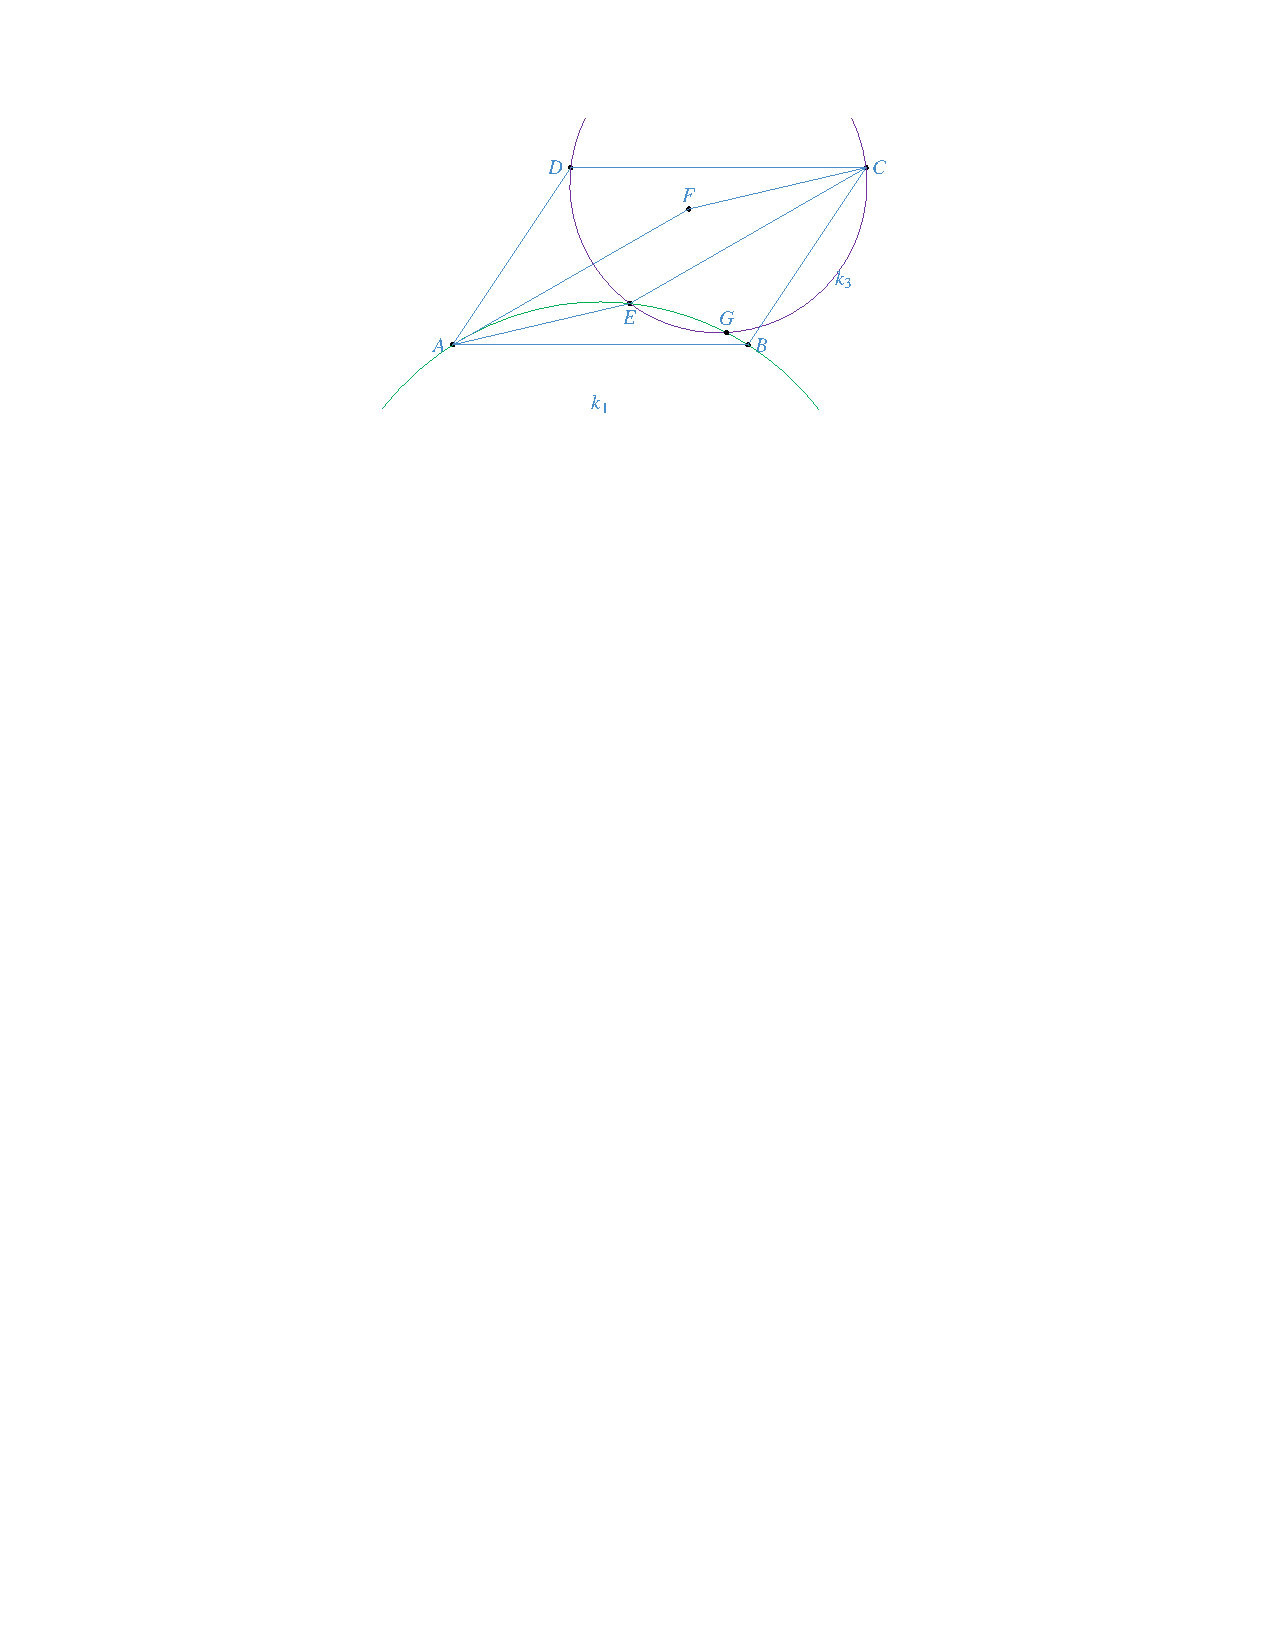
\includegraphics[width=1\linewidth]{h3}
		\caption{\small\textit{\color{cackithi}Hình $2$: Trường hợp $1b$.}}
		\vspace*{-10pt}
	\end{figure}
	\textit{Trường hợp $1c$}: $E = G$. Khi đó hai đường tròn $k_1$ và $k_3$ sẽ tiếp xúc tại tại $G$. Đường tiếp tuyến chung của $k_1$ và $k_3$ đi qua $G$ sẽ chia góc $BGC$ thành hai phần, ký hiệu là $\beta_1$ và $\beta_2$ như trong hình. Ta có $\beta_1 + \beta_2 = \beta = \angle BGC$.
	\begin{figure}[H]
		\vspace*{-5pt}
		\centering
		\captionsetup{labelformat= empty, justification=centering}
		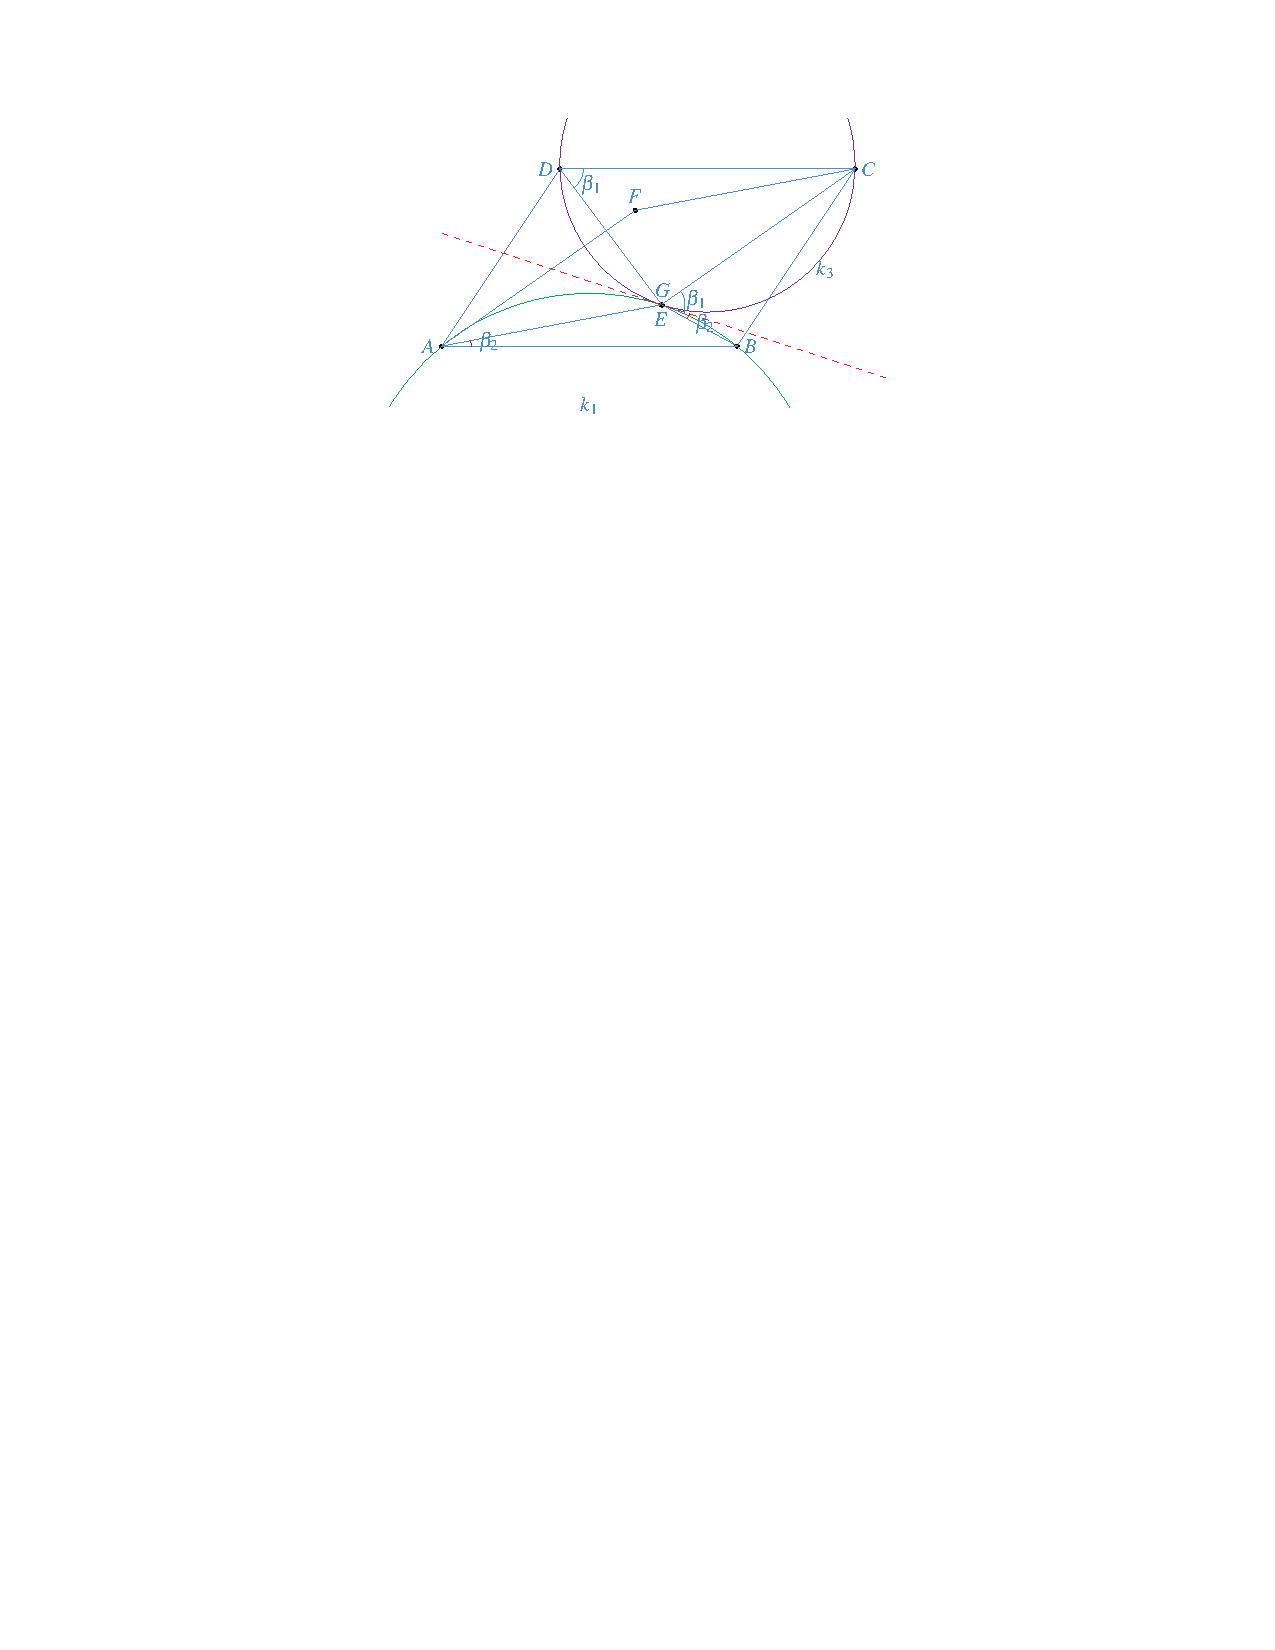
\includegraphics[width=1\linewidth]{h2}
		\caption{\small\textit{\color{cackithi}Hình $3$: Trường hợp $1c$.}}
		\vspace*{-10pt}
	\end{figure}	
	Bằng định lý về góc tạo bởi tia tiếp tuyến và dây cung ta có $\beta_1 = \angle EDC$ và $\beta_2 = \angle EAB$. Do 
	$
	\angle EDC + \angle EAD + \angle EAB + \angle EDA = \angle CDA + \angle DAB = 180^{\circ}
	$
	nên $\angle EDA + \angle EAD =  180^{\circ} - (\angle EDC + \angle EAB) =  180^{\circ} - (\beta_1 + \beta_2) = 180^{\circ} - \beta$. 
	\vskip 0.1cm
	Mặt khác, do $\angle DEA +  \angle EDA + \angle EAD =  180^{\circ}$ nên $\delta = \angle DEA = 180^{\circ} - (\angle EDA + \angle EAD) = 180^{\circ} - (180^{\circ} - \beta) = \beta$. Như vậy $ \angle BGC = \beta = \delta$ và ta có điều phải chứng minh.
	\vskip 0.1cm
	\textbf{\color{cackithi}Trường hợp $2$}: $G$ nằm ngoài $ABCD$. Có thể thấy rằng $G$ không nằm trong vùng tạo bởi hai đường thẳng $AB$ và $CD$, cũng như không nằm trong vùng tạo bởi hai đường thẳng $AD$ và $BC$. Không mất tính tổng quát ta có thể giả sử $G$ nằm gần $B$ như trong hình. Gọi $H$ là điểm đối xứng với $G$ qua tâm $S$. Khi đó hai hình bình hành $AGCH$ và $ABCD$ có chung đường chéo $AC$ với $B,D$ nằm bên trong $AGCH$. Hơn nữa, đường tròn ngoại tiếp của $GBA$ và $GDC$ giao nhau tại điểm $E$ nằm phần trong của $AGCH$.
	\begin{figure}[H]
		\vspace*{-5pt}
		\centering
		\captionsetup{labelformat= empty, justification=centering}
		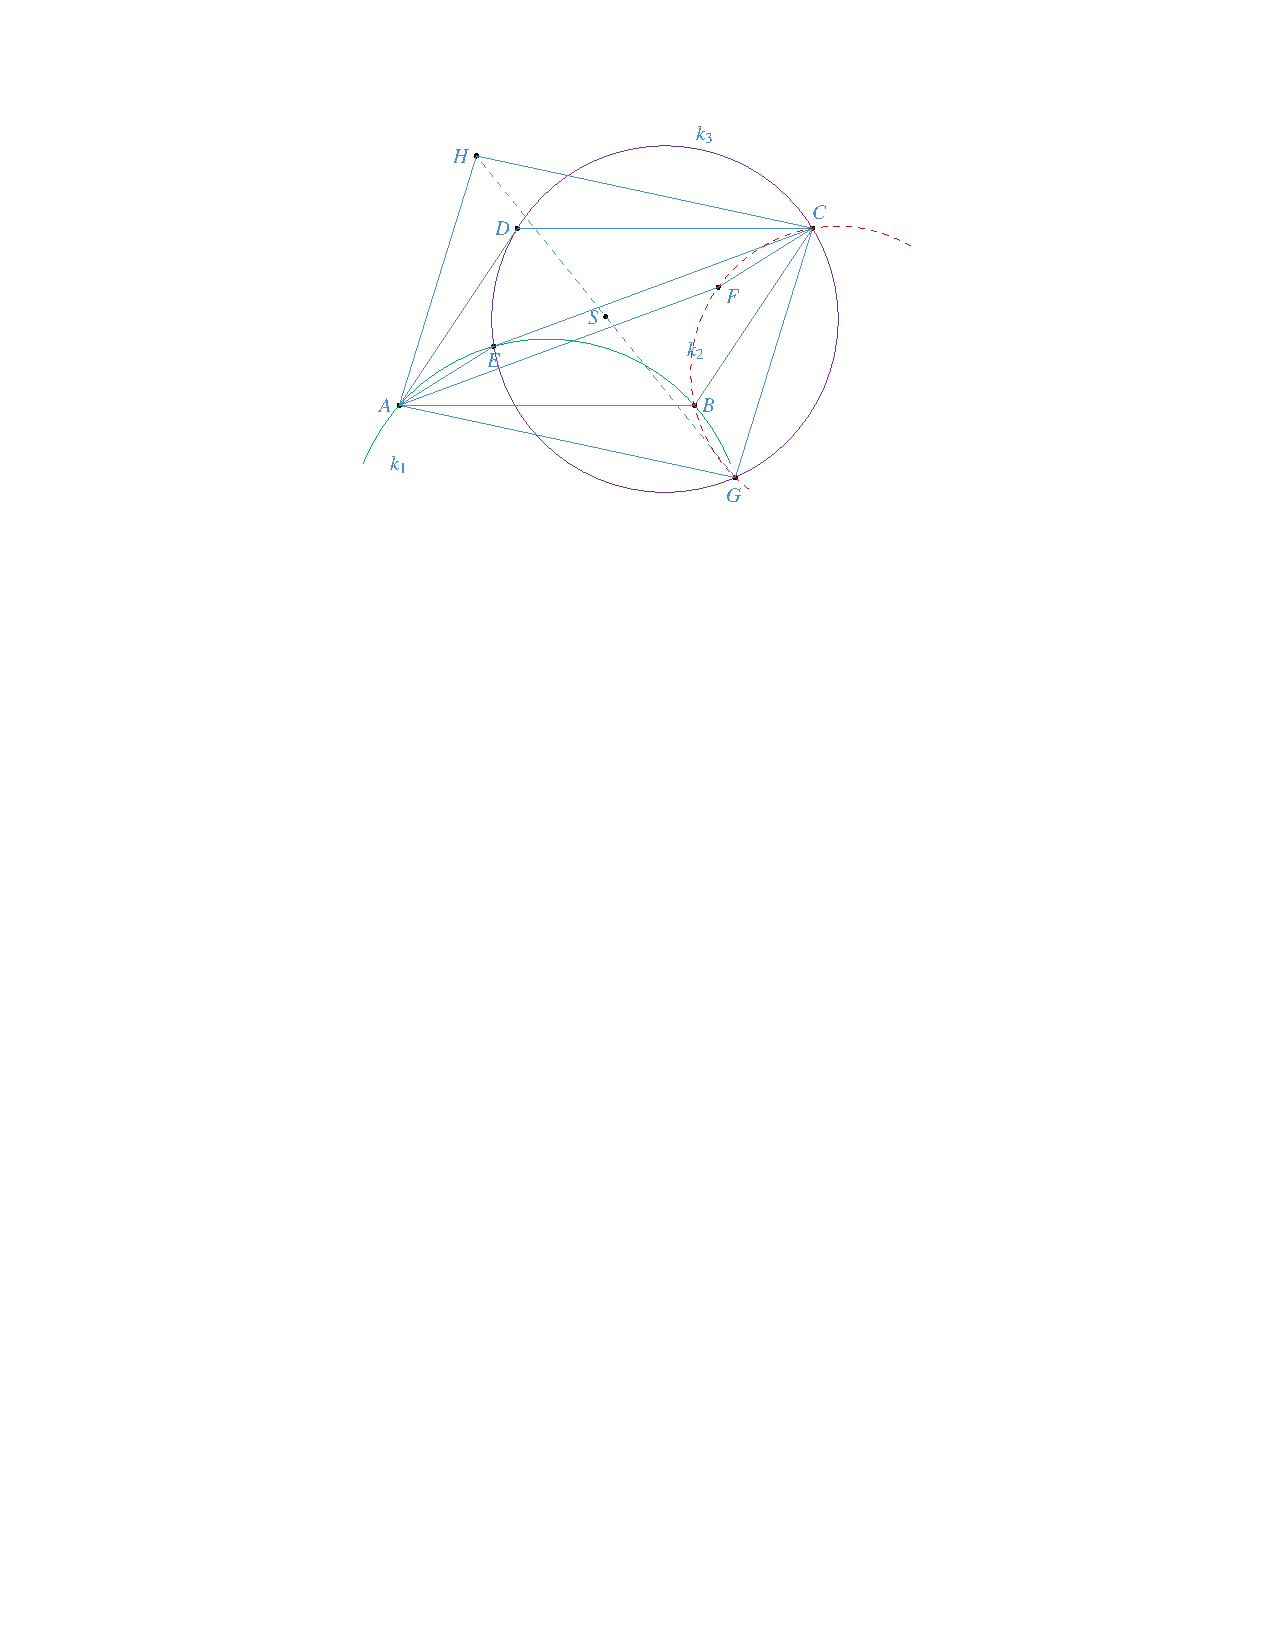
\includegraphics[width=1\linewidth]{h4}
		\caption{\small\textit{\color{cackithi}Hình $4$: Trường hợp $2$.}}
		\vspace*{-10pt}
	\end{figure}
	Sử dụng kết quả của trường hợp $1$ với $AGCH$ thay cho $ABCD$, $ABCD$ cho $AECF$, $GBA$ cho $k_1$, $GDC$ cho $k_2$ ta chứng minh được rằng $E$ thuộc đường tròn $CBH$ và $HDA$. Do tính đối xứng tâm qua $S$ nên $F$ thuộc đường tròn $DAG$ và $GBC$. Do đó, $G$ cũng thuộc đường tròn $DFA$ và $BCF$. Nói cách khác, bốn đường tròn $AFD$, $BFC$, $CED$ và $DFA$ giao nhau tại $G$.
	\vskip 0.1cm
	\textbf{\color{cackithi}Câu $\pmb{4}$}: Cho số thực $\alpha$ với biểu diễn thập phân $\alpha = 0,a_1 a_2 a_3 \ldots$ trong đó mỗi chữ số $a_i$ là một số nguyên tố. Các chữ số sau dấu phẩy được sắp xếp dọc theo đường được tạo ra bởi các mũi tên như trong hình bên, được tưởng tượng là tiếp tục vô tận về bên phải và xuống dưới.
	\vskip 0.1cm
	Với mỗi $m \ge 1$, biểu diễn thập phân của số thực $z_m$ được cho bằng cách viết chữ số $0$ trước dấu phẩy và sau dấu phẩy là các chữ số của dòng thứ $m$ (tính từ trên xuống) theo thứ tự từ trái sang phải. Tương tự, với mọi $n \ge 1$, số thực $s_n$ được thiết lập với các chữ số của cột thứ $n$ (tính từ bên trái sang) theo thự tự từ trên xuống dưới. Chẳng hạn $z_3 = 0, a_5a_6a_7a_{12}a_{23}a_{28}\ldots$ và $s_2 = 0,a_2a_3a_6a_{15}a_{18}a_{35}\ldots$. Chứng minh rằng:
	\vskip 0.1cm
	$(a)$ Nếu $\alpha$ là số hữu tỷ, thì tất cả các số $z_m$ và $s_n$ đều hữu tỷ.
	\vskip 0.1cm
	$(b)$ Chiều ngược lại của khẳng định $(a)$ là sai.
	\vskip 0.1cm
	\textit{Chứng minh.}
	\begin{figure}[H]
		\vspace*{-5pt}
		\centering
		\captionsetup{labelformat= empty, justification=centering}
		\begin{tikzpicture}[cackithi]
			\node (A1) at (0, 0) {$a_1$};
			\node (A2) at (1, 0) {$a_2$};
			\node (A3) at (1, -1) {$a_3$};
			\node (A4) at (0, -1) {$a_4$};
			\node (A5) at (0, -2) {$a_5$};
			\node (A6) at (1, -2) {$a_6$};
			\node (A7) at (2, -2) {$a_7$};
			\node (A8) at (2, -1) {$a_8$};
			\node (A9) at (2, 0) {$a_9$};
			\node (A10) at (3, 0) {$a_{10}$};
			\node (A11) at (3, -1) {$a_{11}$};
			\node (A12) at (3, -2) {$a_{12}$};
			\node (A13) at (3, -3) {$a_{13}$};
			\node (A14) at (2, -3) {$a_{14}$};
			\node (A15) at (1, -3) {$a_{15}$};
			\node (A16) at (0, -3) {$a_{16}$};
			\node (A17) at (0, -4) {$a_{17}$};
			\node (A18) at (1, -4) {$a_{18}$};
			\node (A19) at (2, -4) {$a_{19}$};
			\node (A20) at (3, -4) {$a_{20}$};
			\node (A21) at (4, -4) {$a_{21}$};
			\node (A22) at (4, -3) {$a_{22}$};
			\node (A23) at (4, -2) {$a_{23}$};
			\node (A24) at (4, -1) {$a_{24}$};
			\node (A25) at (4, 0) {$a_{25}$};
			\node (A26) at (5, 0) {$a_{26}$};
			\node (A27) at (5, -1) {$a_{27}$};
			\node (A28) at (5, -2) {$a_{28}$};
			
			\tkzDefPoint(5,-3){A29}
			\tkzDefPoint(5,-5){A31}
			
			% arrows
			\draw[-stealth]
			(A1) edge (A2) (A2) edge (A3) (A3) edge (A4)
			(A4) edge (A5) (A5) edge (A6) (A6) edge (A7)
			(A7) edge (A8) (A8) edge (A9) (A9) edge (A10)
			(A10) edge (A11) (A11) edge (A12) (A12) edge (A13)
			(A13) edge (A14) (A14) edge (A15) (A15) edge (A16)
			(A16) edge (A17) (A17) edge (A18) (A18) edge (A19)
			(A19) edge (A20) (A20) edge (A21) (A21) edge (A22)
			(A22) edge (A23) (A23) edge (A24) (A24) edge (A25)
			(A25) edge (A26) (A26) edge (A27) (A27) edge (A28);
			
			\draw[thick, dotted] (A28) -- (A29);
		\end{tikzpicture}
		\caption{\small\textit{\color{cackithi}Hình $5$:Biểu diễn thập phân của $\alpha$.}}
		\vspace*{-10pt}
	\end{figure}	
	Một số thực với biểu diễn thập phân $\alpha = 0,a_1a_2a_3\ldots$ là hữu tỷ khi và chỉ khi biểu diễn này hữu hạn hoặc tuần hoàn, nghĩa là tồn tại các số nguyên dương $N, p$ sao cho với mọi $i \ge N$ thì $a_{i + p} = a_i$. Số $p$ nhỏ nhất thỏa mãn điều kiện trên được gọi là độ dài của chu kỳ. Mọi số $p$ thỏa mãn điều kiện trên đều là bội số của độ dài chu kỳ. Số $a_{i}$ với $i \ge N$ được gọi là nằm trong phần tuần hoàn (trong biểu diễn thập phân) của $\alpha$. Chẳng hạn, số $\frac{2}{9} = 0,22222 \ldots$ có độ dài chu kỳ là $1$ và phần tuần hoàn bắt đầu ngay sau dấu phẩy, trong khi đó $\frac{3227}{5550} = 0,58144144144 \ldots$ có độ dài chu kỳ $2$ và phần tuần hoàn bắt đầu từ vị trí thứ ba sau dấu phẩy. Vì $0$ và $9$ không xuất hiện trong các biểu diễn thập phân nên các số $\alpha$, $z_m$ và $s_n$ là vô tỷ hoặc tuần hoàn.
	\vskip 0.1cm	
	Gọi chỉ số của chữ số trong biểu diễn thập phân của $\alpha$ tại dòng $r$ cột $s$ như trong hình là $b(r,s)$, chẳng hạn $b(2,2) = 3$ và $b(3,5) = 23$. Như vậy,
		\begin{align*}
			z_m & = 0, a_{b(m,1)} a_{b(m,2)} a_{b(m,3)} a_{b(m,4)} \ldots \\
			s_n & = 0, a_{b(1,n)} a_{b(2,n)} a_{b(3,n)} a_{b(4,n)} \ldots
		\end{align*}
	\begin{figure}[H]
		\vspace*{-5pt}
		\centering
		\captionsetup{labelformat= empty, justification=centering}
		\begin{tikzpicture}[cackithi]
			\node (R1) at (0, 1) {$s = 1$};
			\node (R2) at (1, 1) {$2$};
			\node (R3) at (2, 1) {$3$};
			\node (R4) at (3, 1) {$4$};
			\node (R5) at (4, 1) {$5$};
			\node (R6) at (5, 1) {$6$};
			\node (S1) at (-1, 0) {$r = 1$};
			\node (S2) at (-1, -1) {$2$};
			\node (S3) at (-1, -2) {$3$};
			\node (S4) at (-1, -3) {$4$};
			\node (S5) at (-1, -4) {$5$};
			\node (A1) at (0, 0) {$a_1$};
			\node (A2) at (1, 0) {$a_2$};
			\node (A3) at (1, -1) {$\textcolor{red}{a_3}$};
			\node (A4) at (0, -1) {$a_4$};
			\node (A5) at (0, -2) {$a_5$};
			\node (A6) at (1, -2) {$a_6$};
			\node (A7) at (2, -2) {$a_7$};
			\node (A8) at (2, -1) {$a_8$};
			\node (A9) at (2, 0) {$a_9$};
			\node (A10) at (3, 0) {$a_{10}$};
			\node (A11) at (3, -1) {$a_{11}$};
			\node (A12) at (3, -2) {$a_{12}$};
			\node (A13) at (3, -3) {$a_{13}$};
			\node (A14) at (2, -3) {$a_{14}$};
			\node (A15) at (1, -3) {$a_{15}$};
			\node (A16) at (0, -3) {$a_{16}$};
			\node (A17) at (0, -4) {$a_{17}$};
			\node (A18) at (1, -4) {$a_{18}$};
			\node (A19) at (2, -4) {$a_{19}$};
			\node (A20) at (3, -4) {$a_{20}$};
			\node (A21) at (4, -4) {$a_{21}$};
			\node (A22) at (4, -3) {$a_{22}$};
			\node (A23) at (4, -2) {$\textcolor{red}{a_{23}}$};
			\node (A24) at (4, -1) {$a_{24}$};
			\node (A25) at (4, 0) {$a_{25}$};
			\node (A26) at (5, 0) {$a_{26}$};
			\node (A27) at (5, -1) {$a_{27}$};
			\node (A28) at (5, -2) {$a_{28}$};
			
			\tkzDefPoint(5,-3){A29}
			\tkzDefPoint(5,-5){A31}
			
			% arrows
			\draw[-stealth]
			(A1) edge (A2) (A2) edge (A3) (A3) edge (A4)
			(A4) edge (A5) (A5) edge (A6) (A6) edge (A7)
			(A7) edge (A8) (A8) edge (A9) (A9) edge (A10)
			(A10) edge (A11) (A11) edge (A12) (A12) edge (A13)
			(A13) edge (A14) (A14) edge (A15) (A15) edge (A16)
			(A16) edge (A17) (A17) edge (A18) (A18) edge (A19)
			(A19) edge (A20) (A20) edge (A21) (A21) edge (A22)
			(A22) edge (A23) (A23) edge (A24) (A24) edge (A25)
			(A25) edge (A26) (A26) edge (A27) (A27) edge (A28);
			
			\draw[dashed, red] (A1) -- (A3) --(A7) -- (A13) --(A21) --  node {r = s} (A31);
			\draw[thick, dotted] (A28) -- (A29);
		\end{tikzpicture}
		\caption{\small\textit{\color{cackithi}Hình $6$: Hàng và cột trong biểu diễn của $\alpha$.}}
		\vspace*{-10pt}
	\end{figure}
	Không khó để thấy
		\begin{align*}
			b(1,s) = 
			\begin{cases}
				s^2 & \text{ nếu } s \text{ lẻ,} \\
				(s-1)^2 + 1 & \text{ nếu } s \text{ chẵn}.
			\end{cases}
		\end{align*}
		Từ đó ta có
		\begin{align*} 
			&b(r,s)\\
			 =& 
			\begin{cases}
				\!\!s^2 \!-\! (r\!-\!1) &\!\!\! \text{ nếu } s \text{ lẻ và } s \ge r, \\
				\!\!(s\!-\!1)^2 \!+\! r &\!\!\! \text{ nếu } s \text{ chẵn và } s \ge r.
			\end{cases}\tag{$3$}
		\end{align*}
		Tương tự,
		\begin{align*}
			b(r,1) = 
			\begin{cases}
				(r-1)^2 + 1 & \text{ nếu } r \text{ lẻ,} \\
				r^2 & \text{ nếu } r \text{ chẵn}
			\end{cases}
		\end{align*}
		và 
		\begin{align*}
			&b(r,s) \\
			= 
			&\begin{cases}
				\!\!(r\!-\!1)^2 \!+\! s &\!\!\! \text{ nếu } r \text{ lẻ và } r \ge s, \\
				\!\!r^2 \!-\! (s\!-\!1) &\!\!\!\text{ nếu } r \text{ chẵn và } r \ge s.
			\end{cases}\tag{$4$}
		\end{align*}
		Như vậy, nếu cố định $r$ thì $b(r,s)$ là hàm tăng chặt theo $s$ khi $s \ge r$. Tương tự, nếu $s$ cố định thì $b(r,s)$ là hàm tăng chặt theo $r$ khi $r \ge s$.
		\vskip 0.1cm
		$a.$ Giả sử rằng $\alpha$ là số hữu tỷ. Khi đó, tồn tại cặp số $(N,p)$ sao cho với mọi $i \ge N$ và $K \in \mathbb{N}$ ta có $a_{i + K.p} = a_i$. Ta sẽ chứng minh rằng $z_m$ và $s_n$ là các số tuần hoàn với độ dài chu kỳ là ước số của $2p$.
		\vskip 0.1cm
		Thật vậy, với dòng thứ $m$, gọi $s(m)$ là chỉ số của cột nằm bên phải cột thứ $m$ (do đó $s(m) \ge m$) sao cho $a_{b(m,s(m))}$ nằm trong phần tuần hoàn của $\alpha$. Số $s(m)$ như vậy tồn tại bởi tính tăng chặt của hàm $b(r,s)$ theo $s$ khi $r$ cố định và $s \ge r$. Vì $s$ và $s + 2p$ có cùng tính chẵn lẻ nên từ ($3$) ta có với mọi $s \ge s(m)$: 
		\begin{align*}
			&b(m,s + 2p) - b(m,s) \\
			=& 
			\begin{cases}
				(s + 2p)^2 - s^2 & \text{ nếu } s \text{ lẻ,} \\
				(s +2p -1)^2 - (s-1)^2 & \text{ nếu } s \text{ chẵn}.
			\end{cases} \\
			=&
			\begin{cases}
				2p.(2s + 2p)& \text{ nếu } s \text{ lẻ,} \\
				2p.(2s+2p-2) & \text{ nếu } s \text{ chẵn.}
			\end{cases}
		\end{align*}
		Hiệu số này luôn dương và là bội của $p$, do đó $a_{b(m,s + 2p)} = a_{b(m,s)}$ với mọi $s \ge s(m)$. Vậy ta đã chứng minh rằng tồn tại cặp số nguyên dương $(s(m), 2p)$ sao cho $a_{b(m,s + 2p)} = a_{b(m,s)}$ với mọi $s \ge s(m)$. Nói cách khác, $z_m$ là số tuần hoàn với độ dài chu kỳ là ước của $2p$ với mọi số nguyên dương $m$. 
		\vskip 0.1cm
		Bằng lập luận tương tự, với mỗi $n$, tồn tại số nguyên dương $r(n) \ge n$ sao cho với mọi $r \ge r(n)$ thì hiệu số $b(r + 2p,n) - b(r, n)$ luôn là một bội số dương của $2p$. Do đó, $a_{b(r + 2p,n)} = a_{b(r,n)}$. Vậy $s_n$ là số hữu tỷ với chu kỳ tuần hoàn có độ dài là một ước của $2p$ với mọi số nguyên dương $n$.
		\vskip 0.1cm
		$b.$ Để chứng minh chiều ngược lại của khẳng định $(a)$ là sai, ta chỉ cần chỉ ra một số vô tỷ $\alpha$ sao cho tất cả các số $z_m$ và $s_n$ là hữu tỷ. Thật vậy, chọn 
		\begin{align*}
			&\alpha = \alpha_0 \\
			= &0,22 \ 3 \ 22 \ 333 \ 22 \ 33333 \ 22 \ 33333333 \ 22 \ \ldots
		\end{align*}
		với số $2$ nằm trên hàng và cột đầu tiên còn số $3$ nằm ở các vị trí còn lại như trong Hình $7$. Nói cách khác,
		\begin{align*}
			a_i = 
			\begin{cases}
				2 & \text{ khi }  i = k^2, k^2 + 1, \text{ với } k \in \mathbb{N}, \\
				3 & \text{ ở các vị trí còn lại}.
			\end{cases}
		\end{align*}
		Dễ thấy rằng $z_1 = s_1 = 0,222222 \ldots = \frac{2}{9}$ và $z_m = s_n = 0,233333 \ldots = \frac{7}{30}$ là các số hữu tỷ với mọi $m, n \ge 2$. Mặt khác, nằm giữa $a_{k^2 + 1} = 2$ và $a_{(k+1)^2} = 2$ có đúng $2k-1$ số $3$. Vì $k$ có thể lớn tùy ý, không tồn tại cặp $(N,p)$ sao cho $a_{i + p} = a_i$ với mọi $i \ge N$. Do đó $\alpha$ là số vô tỷ.
		\begin{figure}[H]
			\vspace*{-5pt}
			\centering
			\captionsetup{labelformat= empty, justification=centering}
			\begin{tikzpicture}[cackithi]
				\node (A1) at (0, 0) {$2$};
				\node (A2) at (1, 0) {$2$};
				\node (A3) at (1, -1) {$3$};
				\node (A4) at (0, -1) {$2$};
				\node (A5) at (0, -2) {$2$};
				\node (A6) at (1, -2) {$3$};
				\node (A7) at (2, -2) {$3$};
				\node (A8) at (2, -1) {$3$};
				\node (A9) at (2, 0) {$2$};
				\node (A10) at (3, 0) {$2$};
				\node (A11) at (3, -1) {$3$};
				\node (A12) at (3, -2) {$3$};
				\node (A13) at (3, -3) {$3$};
				\node (A14) at (2, -3) {$3$};
				\node (A15) at (1, -3) {$3$};
				\node (A16) at (0, -3) {$2$};
				\node (A17) at (0, -4) {$2$};
				\node (A18) at (1, -4) {$3$};
				\node (A19) at (2, -4) {$3$};
				\node (A20) at (3, -4) {$3$};
				\node (A21) at (4, -4) {$3$};
				\node (A22) at (4, -3) {$3$};
				\node (A23) at (4, -2) {$3$};
				\node (A24) at (4, -1) {$3$};
				\node (A25) at (4, 0) {$2$};
				\node (A26) at (5, 0) {$2$};
				\node (A27) at (5, -1) {$3$};
				\node (A28) at (5, -2) {$3$};
				
				\tkzDefPoint(5,-3){A29}
				
				
				% arrows
				\draw[-stealth]
				(A1) edge (A2) (A2) edge (A3) (A3) edge (A4)
				(A4) edge (A5) (A5) edge (A6) (A6) edge (A7)
				(A7) edge (A8) (A8) edge (A9) (A9) edge (A10)
				(A10) edge (A11) (A11) edge (A12) (A12) edge (A13)
				(A13) edge (A14) (A14) edge (A15) (A15) edge (A16)
				(A16) edge (A17) (A17) edge (A18) (A18) edge (A19)
				(A19) edge (A20) (A20) edge (A21) (A21) edge (A22)
				(A22) edge (A23) (A23) edge (A24) (A24) edge (A25)
				(A25) edge (A26) (A26) edge (A27) (A27) edge (A28);
				
				\draw[thick, dotted] (A28) -- (A29);
				
			\end{tikzpicture}
			\caption{\small\textit{\color{cackithi}Hình $7$: Biểu diễn thập phân của $\alpha_0$.}}
			\vspace*{-5pt}
		\end{figure}
\end{multicols}
\newpage
\begingroup
\AddToShipoutPicture*{\put(150,700){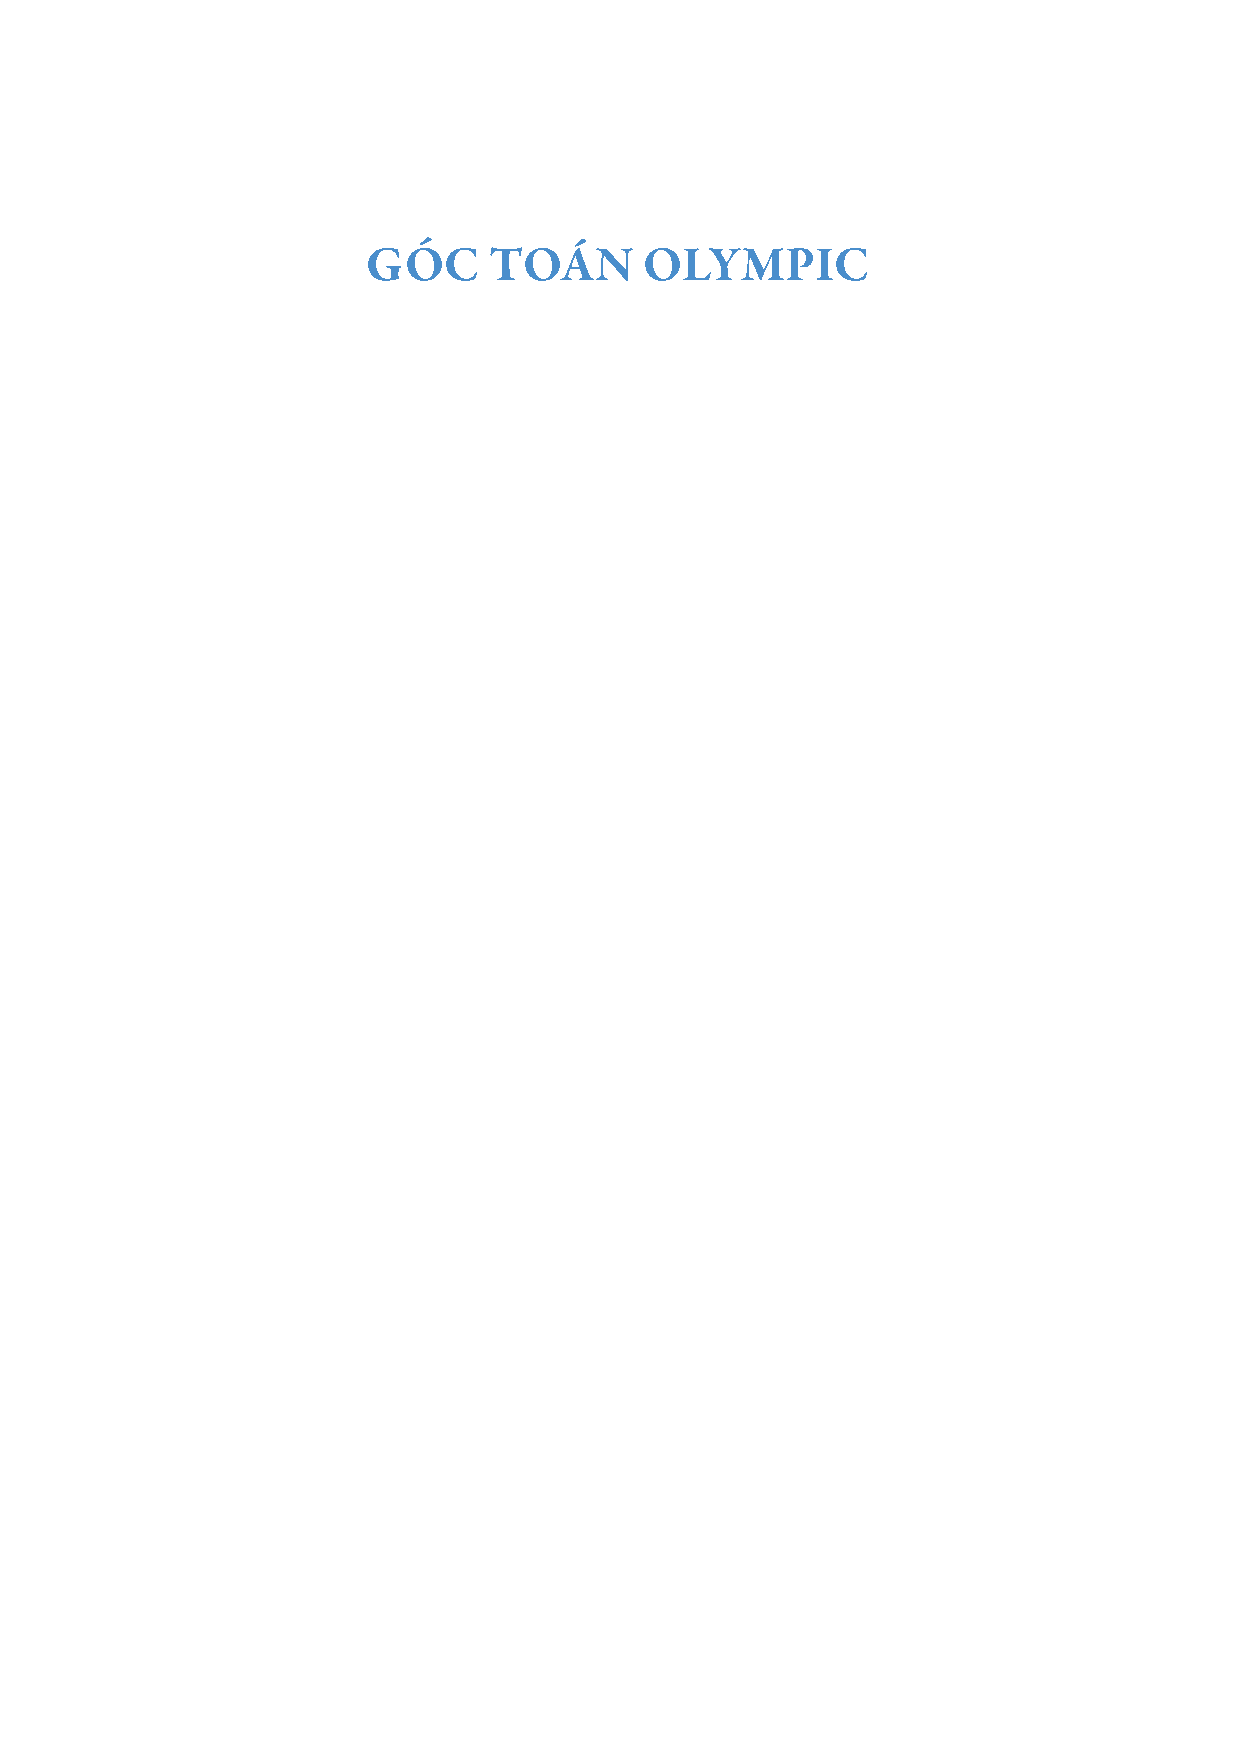
\includegraphics[scale=1]{../tieude1.pdf}}}
\centering
\endgroup
\vspace*{5pt}

\begin{multicols}{2}
	Trong phần đầu chuyên mục, chúng tôi sẽ trình bày lời giải của các bài toán trong kỳ thi Olympic Toán học trẻ của Áo năm $2022$ đăng trong số báo $6/2022$. 
	\begin{figure}[H]
		\vspace*{-5pt}
		\centering
		\captionsetup{labelformat= empty, justification=centering}
		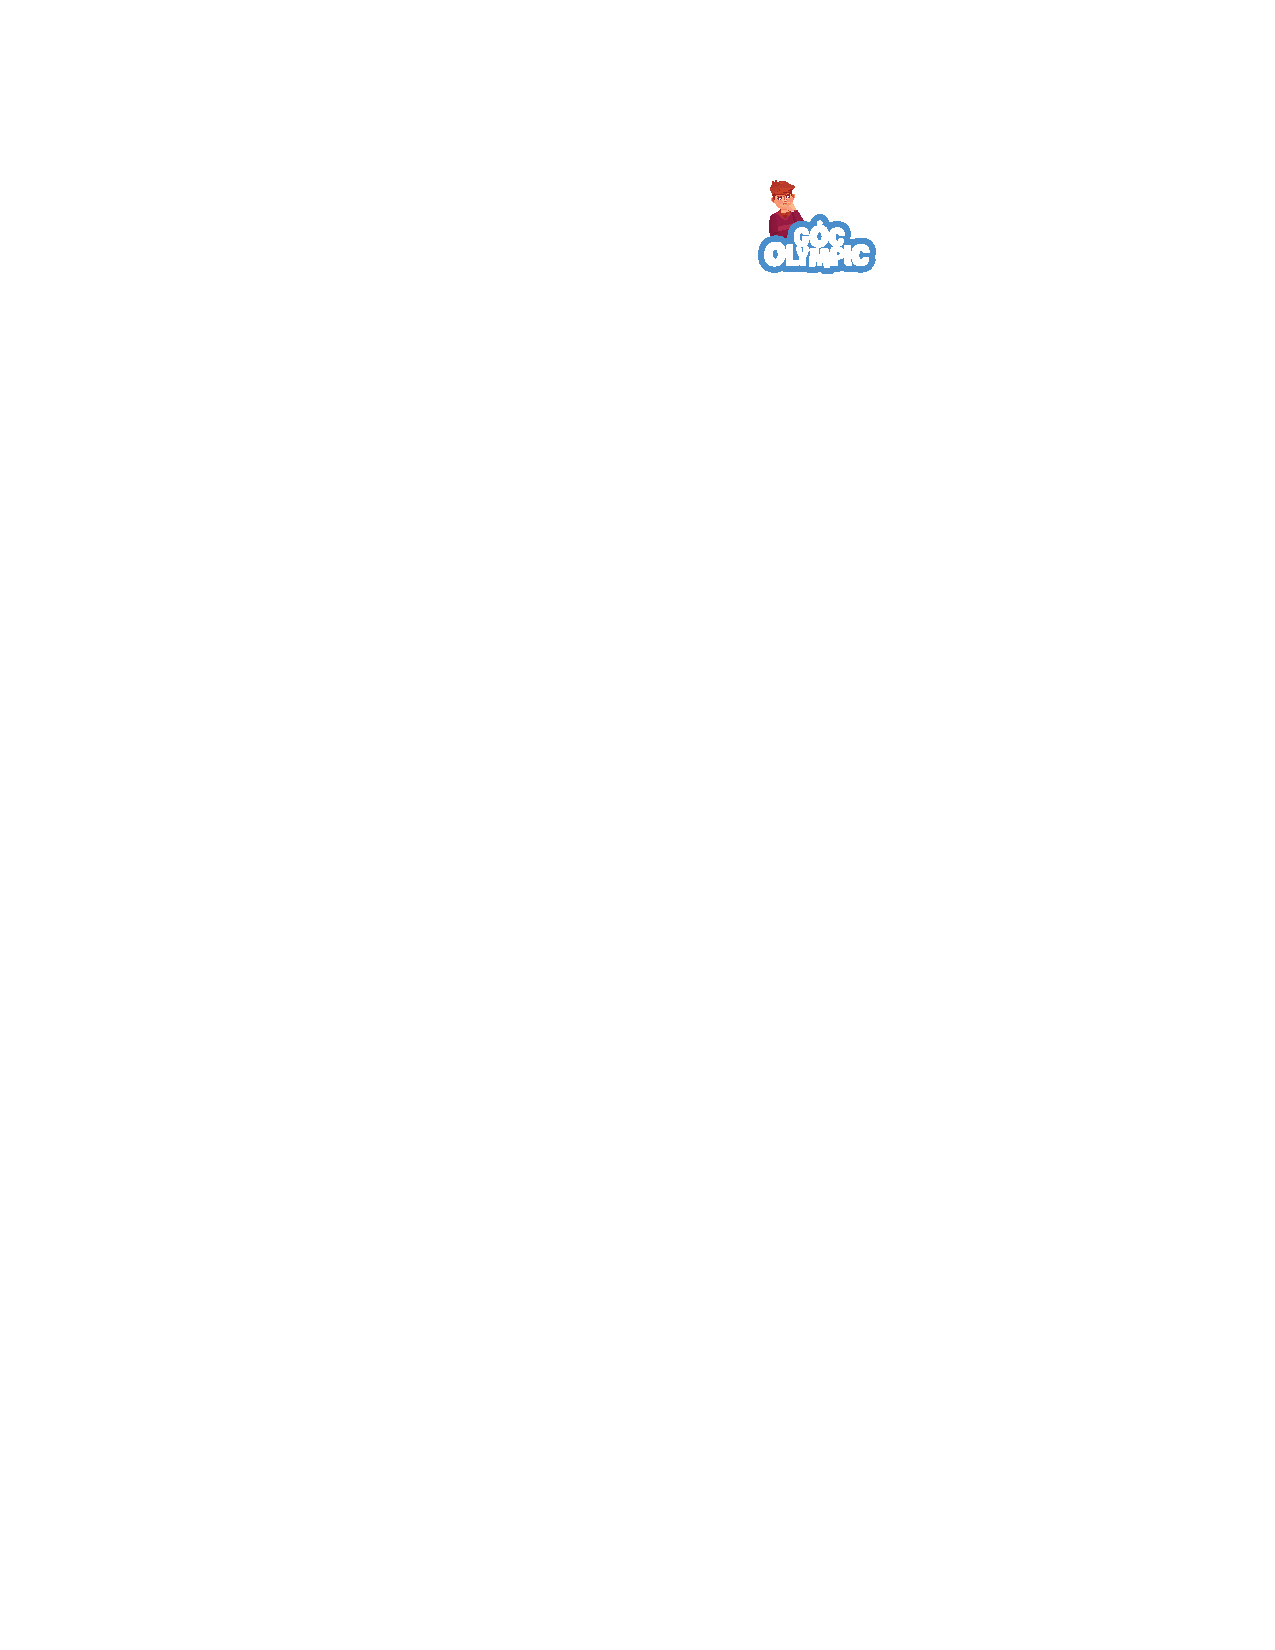
\includegraphics[width= 0.85\linewidth]{gocolympic}
%		\caption{\small\textit{\color{}}}
		\vspace*{-10pt}
	\end{figure}
	{\bf\color{cackithi} OC$\pmb{43.}$} Người ta muốn lát kín một bảng ô vuông kích thước $2\times 13$ ($2$ hàng, $13$ cột) bằng các tấm bìa kích thước $1\times 2$ và $1\times 3$ sao cho các tấm bìa không được chồng lên nhau hay phủ ra ngoài bảng. Có bao nhiêu cách lát nếu ta được phép xoay các tấm bìa nhưng cạnh dài của tất cả các tấm đều phải song song với nhau? (số lượng mỗi tấm không hạn chế).   
	\vskip 0.1cm
	\textit{Lời giải.} Theo giả thiết trong đầu bài, ta chỉ cần xét $2$ trường hợp:
	\vskip 0.1cm
	Trường hợp $1$: các tấm bìa đều xếp thẳng đứng. Như vậy chỉ có thể dùng các tấm $1\times 2$  và trường hợp này chỉ có đúng $1$ cách lát.
	\vskip 0.1cm
	Trường hợp $2$: các tấm bìa đều xếp nằm ngang. Trước tiên ta đếm số cách lát một hàng ngang gồm $13$ ô vuông. Gọi $x$ là số tấm độ dài $2$ và $y$ là số tấm độ dài $3$ thì $2x+3y=13.$ Ta dễ dàng thấy phương trình có $2$ nghiệm nguyên không âm là $(x,y)=(2,3)$ và $(x,y)=(5,1).$ Với trường hợp $(x,y)=(2,3)$ ta có $5$ tấm và một cách lát sẽ được xác định duy nhất bởi thứ tự các tấm trên hàng ngang. Như vậy trong trường hợp này, số cách lát bằng số cách chọn ra $2$ vị trí đặt các tấm $1\times 2$ trong số $5$ vị trí và bằng ${5 \choose 2}=10.$  Lý luận tương tự, trường hợp  $(x,y)=(5,1)$ có  ${6 \choose 5}=6$ cách lát. Tổng cộng ta có $16$ cách lát một hàng ngang. Do đó, theo quy tắc nhân, trong trường hợp $2$ ta có $16^2=256$ cách lát.
	\vskip 0.1cm
	Tổng cộng cả hai trường hợp, ta nhận được đáp số là $257$ cách lát thỏa mãn yêu cầu trong bài. 
	\vskip 0.1cm
	{\bf\color{cackithi} OC$\pmb{44.}$} Cho đoạn thẳng $AB$ với trung điểm $M.$ Dựng nửa đường tròn tâm $M$, đường kính $AB$. Cho $P$ là một điểm trên nửa đường tròn ($P$ khác với $A, B$)  và $Q$ là trung điểm của cung  $AP.$ Gọi  giao điểm của đường thẳng $BP$ với đường thẳng đi qua $M$ song song $PQ$ là  $S.$
	Chứng minh rằng $PM = PS.$
	\vskip 0.1cm
	\textit{Lời giải.}
	\begin{figure}[H]
		\vspace*{-15pt}
		\centering
		\captionsetup{labelformat= empty, justification=centering}
		\begin{tikzpicture}[cackithi, scale=0.85]
	\draw [shift={(3.,0.)}] (0,0) -- (109.18374269243076:0.4) arc (109.18374269243076:180.:0.4) -- cycle;
	\draw [shift={(6.,0.)}] (0,0) -- (109.18374269243077:0.4) arc (109.18374269243077:180.:0.4) -- cycle;
	\draw[] (2.5831269967609543,1.198190773075248) -- (2.3159906402340478,1.10524903314356) -- (2.408932380165736,0.8381126766166536) -- (2.6760687366926423,0.9310544165483414) -- cycle; 
	\draw[] (5.085001116858378,1.7691670931649948) -- (5.177942856790066,1.5020307366380883) -- (5.445079213316973,1.5949724765697764) -- (5.352137473385285,1.8621088330966828) -- cycle; 
	\draw [shift={(3.,0.)}] (0,0) -- (38.36748538486153:0.3) arc (38.36748538486153:109.18374269243076:0.3) -- cycle;
	\draw [shift={(3.,0.)}] (0,0) -- (-16.22438596135386:0.54) arc (-16.22438596135386:38.36748538486152:0.54) -- cycle;
	\draw [shift={(3.,0.)}]  plot[domain=0.:3.141592653589793,variable=\t]({1.*3.*cos(\t r)+0.*3.*sin(\t r)},{0.*3.*cos(\t r)+1.*3.*sin(\t r)});
	\draw  (0.,0.)-- (6.,0.);
	\draw  (5.352137473385285,1.8621088330966828)-- (0.,0.);
	\draw  (2.0142039815854034,2.8334089380246414)-- (3.,0.);
	\draw  (2.0142039815854034,2.8334089380246414)-- (5.352137473385285,1.8621088330966828);
	\draw  (3.,0.)-- (6.337933491799883,-0.9713001049279592);
	\draw  (6.337933491799883,-0.9713001049279592)-- (5.352137473385285,1.8621088330966828);
	\draw [dashed] (3.,0.)-- (5.352137473385285,1.8621088330966828);
	\draw [shift={(3.,0.)}] (-16.22438596135386:0.54) arc (-16.22438596135386:38.36748538486152:0.54);
	\draw [shift={(3.,0.)}] (-16.22438596135386:0.41) arc (-16.22438596135386:38.36748538486152:0.41);
		\draw [fill=white] (0.,0.) circle (1.6pt);
		\draw (-0.28,-0.21) node {$A$};
		\draw [fill=white] (6.,0.) circle (1.6pt);
		\draw (6.28,0.25) node {$B$};
		\draw [fill=white] (3.,0.) circle (1.6pt);
		\draw (2.88,-0.43) node {$M$};
		\draw [fill=white] (5.352137473385285,1.8621088330966828) circle (1.6pt);
		\draw (5.58,2.27) node {$P$};
		\draw [fill=white] (2.6760687366926423,0.9310544165483414) circle (1.6pt);
		\draw [fill=white] (2.0142039815854034,2.8334089380246414) circle (1.6pt);
		\draw (1.96,3.27) node {$Q$};
		\draw [fill=white] (6.337933491799883,-0.9713001049279592) circle (1.6pt);
		\draw (6.62,-0.95) node {$S$};
\end{tikzpicture}
		\vspace*{-10pt}
	\end{figure} 
	Vì $Q$ là trung điểm của cung $AP$ nên $MQ$ vuông góc với $AP.$ Vì đường thẳng $BP$ cũng vuông góc với $AP$, nên suy ra rằng hai đường thẳng $MQ$ và $BP$ song song với nhau. Hơn nữa, theo giả thiết $MS$ và $PQ$ song song với nhau nên tứ giác là $MSPQ$ là  hình bình hành. Do đó $PS = QM = PM$, vì $QM, PM$ là bán kính đường tròn. Ta nhận được điều phải chứng minh.
	\vskip 0.1cm
	{\bf\color{cackithi} OC$\pmb{45.}$} Tìm tất các các số nguyên tố $p, q$ và $r$ thỏa mãn $p +q^2=r^4.$
	\vskip 0.1cm
	\textit{Lời giải.} 
	Ta có thể viết lại đẳng thức trong đầu bài dưới dạng $p = r^4 - q^2 = (r^2 - q)(r^2 + q).$
	Vì $p$ là số nguyên tố nên từ đẳng thức trên ta suy ra $r^2 - q = 1$ và $r^2 + q = p.$ Từ $r^2 - q = 1$ ta có $q = r^2 - 1 = (r - 1)(r + 1).$
	Vì $q$ là số nguyên tố nên ta  lại có $r - 1 = 1$ hay $r = 2$ và $q = 3.$ Do $r^2 + q = p$ ta có $p = 7.$
	\vskip 0.1cm	
	Trong phần cuối của chuyên mục kỳ này, chúng tôi sẽ giới thiệu với bạn đọc ba bài toán trong cuộc thi  Cúp Toán học Châu Âu năm $2022$. Đây là một cuộc thi toán dành cho học sinh THPT và cuối cấp THCS được tổ chức bởi Hiệp hội Tài năng Toán học Trẻ mang tên Marin Getaldić của Croatia.  
	\vskip 0.1cm
	{\bf\color{cackithi} OC$\pmb{52.}$} Tìm tất cả các số nguyên dương $n$ thỏa mãn: tồn tại ba ước dương $a, b, c$ của $n,$ với $a > b > c,$ sao cho ba số $a^2-b^2, b^2-c^2, a^2-c^2$ 
	cũng là các ước của $n.$
	\vskip 0.1cm
	{\bf\color{cackithi} OC$\pmb{53.}$} Cho tam giác nhọn $ABC$ với $BC < AC$. Giả sử đường tròn $\tau$ nội tiếp tam giác $ABC$ có tâm $I$ và tiếp xúc với $BC, AC$ lần lượt tại $D, E.$ Lấy điểm $M$ nằm trên đường tròn $\tau$  sao cho $BM$ song song với $DE$ và hai điểm $M, B$  nằm về cùng một phía của đường phân giác góc $BCA.$ Gọi $F$ và $H$ lần lượt là giao điểm (khác $M$) của $\tau$ với $BM$ và $CM.$  Gọi $J$ là một điểm trên đường thẳng $AC$ sao cho $JM$ song song với $EH$. Gọi $K$ là giao điểm (khác $F$) của $JF$ với $\tau.$ 
	Chứng minh hai đường thẳng $ME$ và $KH$ song song.
	\vskip 0.1cm
	{\bf\color{cackithi} OC$\pmb{54.}$} Cho $n \ge 3$ là số nguyên dương. Alice và Bob  chơi một trò chơi trong đó họ thay phiên nhau tô màu các đỉnh của đa giác đều $n$ cạnh. Alice đi đầu tiên. Cả hai người chơi bắt đầu trò chơi với $0$ điểm. Trong mỗi lượt, người chơi chọn một đỉnh $V$ chưa được tô màu và tô màu nó. Sau đó, họ cộng $k$ điểm vào tổng số điểm của mình, trong đó $k$ là số đỉnh nằm cạnh  $V$ đã được tô màu. (Như vậy, $k$ sẽ có giá trị $0$, $1$ hoặc $2$.)
	Trò chơi kết thúc khi tất cả các đỉnh đã được tô màu và người chơi nào có nhiều điểm hơn sẽ thắng. Xác định người chơi nào có chiến lược để luôn chiến thắng
\end{multicols}
\vspace*{-10pt}
{\color{cackithi}\rule{1\linewidth}{1pt}}
\vskip 0.2cm
\centerline{\Large{\textbf{\color{cackithi}LỜI GIẢI, ĐÁP ÁN}}}
\vskip 0.1cm
\begin{multicols}{2}
	\textit{Cách $2$}:
	Ta sẽ dõi theo các Đối trọng -- đó là hiệu số giữa số lượng câu trả lời ``Có" và ``Không" tại từng thời điểm. Quy ước tại thời điểm $t=0$ là khi chưa có ai trả lời, $T=1$ khi người đứng đàu dãy trả lời, \ldots $t=500$ là thời điểm người cuối dãy trả lời.
	\vskip 0.1cm
	Do tổng cộng có $250$ câu trả lời ``Có", $250$ câu trả lời ``Không", tại thời điểm ban đầu và thời điểm cuối, các Đối trọng này đều bằng $0$. Với mỗi câu trả lời mới, Đối trọng sẽ thay đổi thêm hoặc bớt đúng $1$ đơn vị. Các Đối trọng bằng $0$ sẽ chia dãy $500$ thổ dân thành các nhóm. Trong mỗi nhóm các Đối trọng có dấu không đổi. 
	\begin{align*}
		0 + + + + 0 - - &{\color{toanhocdoisong}0 - - - - - - 0} \ldots 0\\
		&\text{\color{toanhocdoisong}một nhóm}
	\end{align*}
	Những người Phụ hoạ luôn làm tăng giá trị tuyệt đối của các Đối trọng. Như vậy, để làm Đối trọng quay về $0$, số các thổ dân sống theo nguyên tắc ở trong mỗi nhóm phải nhiều hơn hoặc bằng số những người Phụ hoạ. Điều này đúng cho mỗi nhóm, do đó cũng đúng cho toàn bộ cả $500$ thổ dân của bộ lạc.
	\vskip 0.1cm
	Sau đây ta đưa ra tình huống mà có đúng $250$ người Phụ hoạ. Giả sử bộ lạc có $250$ người theo nguyên tắc, gồm k người Thật thà và $250-k$ người Nói dối ($k$ tuỳ ý sao cho $125< k<250$), còn lại là $250$ người Phụ hoạ. 
	\vskip 0.1cm
	Ta xếp $k$ người Phụ hoạ đứng đầu tiên, với giả sử người đầu tiên trả lời ``Không", cả $k$ người này sẽ trả lời như nhau là ``Không". Tiếp theo ta xếp $k$ người Thật thà, họ đều trả lời là ``Có". Bây giờ số trả lời ``Không" và ``Có" bằng nhau, nên $250-k$ người Phụ hoạ sẽ được xếp tiếp theo đó với câu trả lời ``Có" như nhau (giả sử người đầu tiên trong số $250-k$ người này trả lời có). Còn lại là $250-k$ người Nói dối với trả lời ``Không" được xếp cuối hàng.
	\vskip 0.1cm
	Đáp số: $250$ người Phụ hoạ.
\end{multicols}